\section{Aulyardha Anindita | 1174054}
\subsection{Menulis Shapefile dengan PySHP}
\begin{enumerate}
	\item Nomor 1
	\lstinputlisting{src/tugas2/1174054/no1.py}
	\begin{figure}[H]
		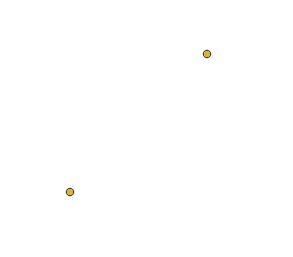
\includegraphics[width=6cm]{figures/Tugas2/1174054/no1.png}
		\centering
		\caption{Point (Titik)}
	\end{figure}
	\item Nomor 2
	\lstinputlisting{src/tugas2/1174054/no2.py}
	\begin{figure}[H]
		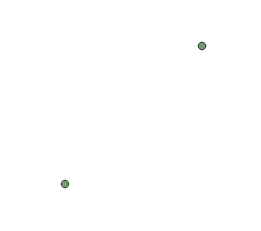
\includegraphics[width=6cm]{figures/Tugas2/1174054/no2.png}
		\centering
		\caption{Point (Titik)}
	\end{figure}
	\item Nomor 3
	\lstinputlisting{src/tugas2/1174054/no3.py}
	\begin{figure}[H]
		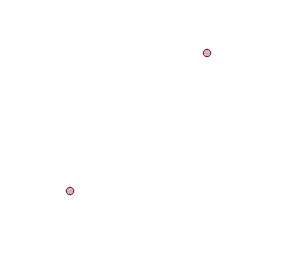
\includegraphics[width=6cm]{figures/Tugas2/1174054/no3.png}
		\centering
		\caption{Point (Titik)}
	\end{figure}
	\item Nomor 4
	\lstinputlisting{src/tugas2/1174054/no4.py}
	\begin{figure}[H]
		
\includegraphics[width=6cm]{figures/Tugas2/1174054/no4.png}
		\centering
		\caption{Point (Titik)}
	\end{figure}
	\item Nomor 5
	\lstinputlisting{src/tugas2/1174054/no5.py}
	\begin{figure}[H]
		
\includegraphics[width=6cm]{figures/Tugas2/1174054/no5.png}
		\centering
		\caption{PolyLine (Garis)}
	\end{figure}
	\item Nomor 6
	\lstinputlisting{src/tugas2/1174054/no6.py}
	\begin{figure}[H]
		
\includegraphics[width=6cm]{figures/Tugas2/1174054/no6.png}
		\centering
		\caption{Polygon (Bidang)}
	\end{figure}
	\item Nomor 7
	\lstinputlisting{src/tugas2/1174054/no7.py}
	\begin{figure}[H]
		
\includegraphics[width=6cm]{figures/Tugas2/1174054/no7.png}
		\centering
		\caption{Polygon (Bidang)}
	\end{figure}
	\item Nomor 8
	\lstinputlisting{src/tugas2/1174054/no8.py}
	\begin{figure}[H]
		
\includegraphics[width=6cm]{figures/Tugas2/1174054/no8.png}
		\centering
		\caption{Polygon (Bidang)}
	\end{figure}
	\item Nomor 9
	\lstinputlisting{src/tugas2/1174054/no9.py}
	\begin{figure}[H]
		
\includegraphics[width=6cm]{figures/Tugas2/1174054/no9.png}
		\centering
		\caption{Polygon (Bidang)}
	\end{figure}
	\item Nomor 10
	\lstinputlisting{src/tugas2/1174054/no10.py}
	\begin{figure}[H]
		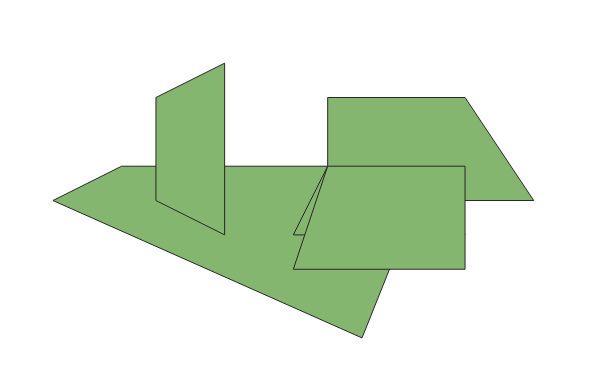
\includegraphics[width=6cm]{figures/Tugas2/1174054/no10.png}
		\centering
		\caption{Polygon, Hasil modulus dari npm saya 1174054 adalah 6 jadi membuat bidang trapesium sebanyak 5 buah trapesium}
	\end{figure}
\end{enumerate}
\subsection{Link}
https://youtu.be/uL6MsNriqmk